\documentclass[a4paper]{article}
\usepackage[pdftex]{hyperref}
\usepackage[latin1]{inputenc}
\usepackage[english]{babel}
\usepackage{a4wide}
\usepackage{amsmath}
\usepackage{amssymb}
\usepackage{algorithmic}
\usepackage{algorithm}
\usepackage{ifthen}
\usepackage{listings}
% move the asterisk at the right position
\lstset{basicstyle=\ttfamily,tabsize=4,literate={*}{${}^*{}$}1}
%\lstset{language=C,basicstyle=\ttfamily}
\usepackage{moreverb}
\usepackage{palatino}
\usepackage{multicol}
\usepackage{tabularx}
\usepackage{comment}
\usepackage{verbatim}
\usepackage{color}

%% pdflatex?
\newif\ifpdf
\ifx\pdfoutput\undefined
\pdffalse % we are not running PDFLaTeX
\else
\pdfoutput=1 % we are running PDFLaTeX
\pdftrue
\fi
\ifpdf
\usepackage[pdftex]{graphicx}
\else
\usepackage{graphicx}
\fi
\ifpdf
\DeclareGraphicsExtensions{.pdf, .jpg}
\else
\DeclareGraphicsExtensions{.eps, .jpg}
\fi

\parindent=0cm
\parskip=0cm

\setlength{\columnseprule}{0.4pt}
\addtolength{\columnsep}{2pt}

\addtolength{\textheight}{5.5cm}
\addtolength{\topmargin}{-26mm}
\pagestyle{empty}

%%
%% Sheet setup
%% 
\newcommand{\coursename}{Machine Learning}
\newcommand{\courseno}{CO22-320372}
 
\newcommand{\sheettitle}{\textbf{Mini-Project}}
\newcommand{\mytitle}{}
\newcommand{\mytoday}{{March 12}, 2019}

% Current Assignment number
\newcounter{assignmentno}
\setcounter{assignmentno}{1}

% Current Problem number, should always start at 1
\newcounter{problemno}
\setcounter{problemno}{1}

%%
%% problem and bonus environment
%%
\newcounter{probcalc}
\newcommand{\problem}[2]{
  \pagebreak[2]
  \setcounter{probcalc}{#2}
  ~\\
  {\large \textbf{{\arabic{assignmentno}}.{\arabic{problemno}}} \hspace{0.2cm}\textit{#1}} \refstepcounter{problemno}\vspace{2pt}\\}

\newcommand{\bonus}[2]{
  \pagebreak[2]
  \setcounter{probcalc}{#2}
  ~\\
  {\large \textbf{Bonus Problem {\arabic{assignmentno}}.{\arabic{problemno}}} \hspace{0.2cm}\textit{#1}} \refstepcounter{problemno}\vspace{2pt}\\}

%% some counters  
\newcommand{\assignment}{\arabic{assignmentno}}

%% solution  
\newcommand{\solution}{\pagebreak[2]{\bf Solution:}\\}

%% Hyperref Setup
\hypersetup{pdftitle={Homework \assignment},
  pdfsubject={\coursename},
  pdfauthor={},
  pdfcreator={},
  pdfkeywords={Computer Networks},
  %  pdfpagemode={FullScreen},
  %colorlinks=true,
  %bookmarks=true,
  %hyperindex=true,
  bookmarksopen=false,
  bookmarksnumbered=true,
  breaklinks=true,
  %urlcolor=darkblue
  urlbordercolor={0 0 0.7}
}

\begin{document}
\coursename \hfill Course: \courseno\\
Jacobs University Bremen \hfill \mytoday\\
{Dragi Kamov \\
Aadil Anil Kumar}\hfill
\vspace*{0.3cm}\\
\begin{center}
{\Large \sheettitle{} {\assignment}\\}
\end{center}

{
{\Large K-Means Clustering:} \\
\begin{enumerate}
	\item {\large Randomly define K centroids}
	\item {\large Assign data points to the closest centroid using standard Euclidean distance}
	\item {\large Calculate the mean values of all points belonging to a centroid, this is the new value of the centroid}
	\item {\large Repeat steps 2 and 3 for specified iterations, causing convergence} \\
\end{enumerate}
}

{
{\textbf{\large K = 1}} \\ \\

\begin{center}
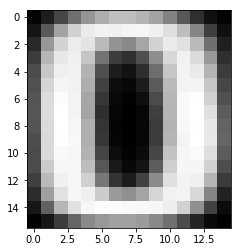
\includegraphics[scale=1.0]{./k1.png}  \\
\end{center}

For the case where K = 1, there is only one cluster that is created. Hence, running many iterations does not make a difference in the convergence of the centroids as it just the mean value of the set. \\ 
We can see this by taking the mean of the zeros vector and then computing the Euclidean Distance from the mean to the centroid of the cluster. (See Jupyter Notebook)\\
\begin{center}
 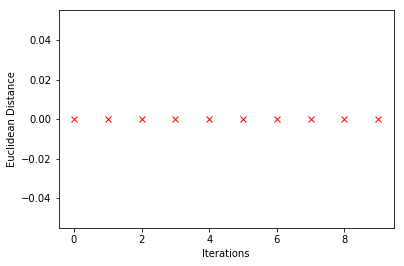
\includegraphics[scale=.80]{./k1plt.png} \\
\end{center} 

\newpage
\textbf{\large K = 2} \\ \\
\begin{center}
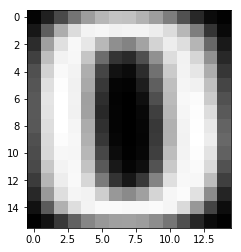
\includegraphics[scale=.85]{./k2_1.png}  \\
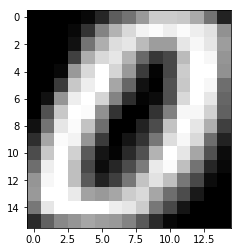
\includegraphics[scale=.85]{./k2_2.png}  \\
\end{center}
For the case of K = 2, there are two clusters that are created. At this point the amount of iterations that are performed matters, as with each iteration the centroids get closer to convergence. However, it converges very quick and the distance from the mean of the vector and centroids stays the same for the rest of the iterations.  \\
\begin{center}
 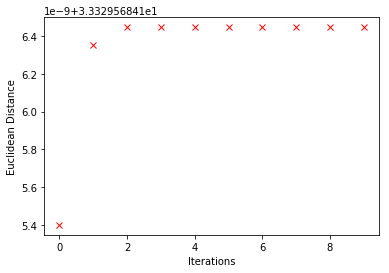
\includegraphics[scale=.80]{./k2plt.png} \\
\end{center} 

\newpage
\textbf{\large K = 3} \\ \\
\begin{center}
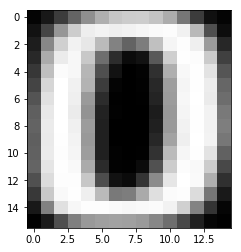
\includegraphics[scale=.85]{./k3_1.png}  \\
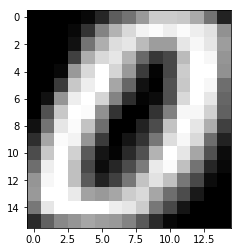
\includegraphics[scale=.85]{./k3_2.png}  
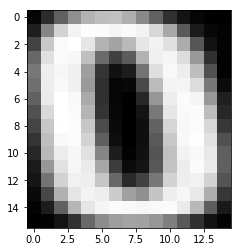
\includegraphics[scale=.85]{./k3_3.png}  \\
\end{center}
For the case of K = 3, there are three clusters that are created. Again as with K = 2, the number of iterations definetly increases the rate of convergence. 
\begin{center}
 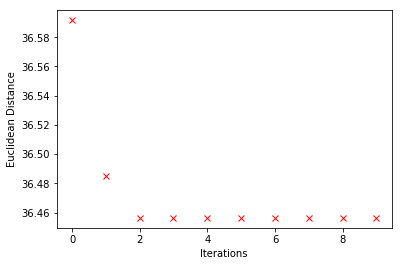
\includegraphics[scale=.80]{./k3plt.png} \\
\end{center} 
}
\newpage
\textbf{\large K = 200} \\ \\
\begin{center}
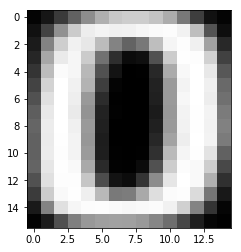
\includegraphics[scale=.85]{./k4_11.png}  \\
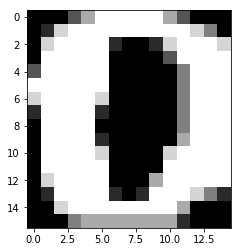
\includegraphics[scale=.85]{./k4_3.png}  
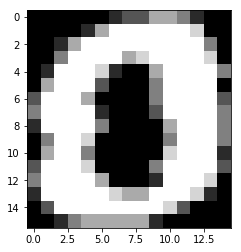
\includegraphics[scale=.85]{./k4_1.png}  \\
\end{center}
For the case of K = 200, there are 200 clusters created. In this case all 200 data points form their own cluster. Iterations do not make a difference as the Euclidean distance stays the same. \\
\begin{center}
 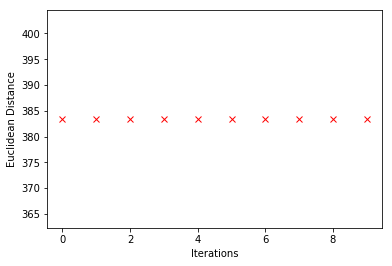
\includegraphics[scale=.80]{./k4plt.png} \\
\end{center} 
\end{document}